\documentclass[10pt, conference, compsocconf]{IEEEtran}
\IEEEoverridecommandlockouts % for \thanks
\usepackage{graphicx}
\usepackage{wrapfig}
\usepackage{url}
%\usepackage{natbib}
%\usepackage{hyperref} -- DISABLED: fails ``PDF express'' check

% \usepackage{authblk} -- must use IEEE's own
% \usepackage[margin=1in]{geometry}

\title{Katana: Towards Patching as a Part of the ELF Toolchain}

\author{\IEEEauthorblockN{Sergey Bratus, James Oakley, Ashwin Ramaswamy, 
Sean W.\ Smith\thanks{The first four authors' work was supported in part by the National
Science Foundation, under grant CNS-0524695.  The views and
conclusions do not necessarily represent those of the sponsors.}}
\IEEEauthorblockA{Computer Science Dept.\\
  Dartmouth College\\
  Hanover, New Hampshire}
\and
\IEEEauthorblockN{Michael E.\ Locasto\thanks{Locasto is supported in part by grant
2006-CS-001-000001 from the U.S. Department of Homeland Security under
the auspices of the I3P research program. The I3P is managed by
Dartmouth College. The opinions expressed in this paper should not be
taken as the view of the authors' institutions, the DHS, or the I3P.}}
\IEEEauthorblockA{Computer Science Dept.\\
George Mason University\\
Arlington, Virginia}}

% correct bad hyphenation here
\hyphenation{op-tical net-works semi-conduc-tor}


\begin{document}

\maketitle
%\pagestyle{plain}

\begin{abstract}
Despite advances in software modularity, security, and reliability,
offline patching remains the predominant form of updating or
protecting commodity software.  Unfortunately, the mechanics of {\it
  hot patching} (the process of upgrading a program while it executes)
remain understudied, even though such a capability offers practical
benefits for both consumer and mission-critical systems.
%
A reliable hot patching procedure would serve particularly well by
reducing the downtime necessary for critical functionality or security
upgrades.  Yet, hot patching also carries the risk -- real or
perceived -- of leaving the system in an inconsistent state, which
leads many owners to forgo its benefits as too risky.  
%
%MEL:
%entity -- an
%application binary, library or even the kernel, while it is still in
%execution. 
%SB:
% It offers enormous benefits as it helps in mitigating
% process downtime and contributes to overall system reliability and
% availability.
%
%It offers great practical benefits for mission-critical systems, by
%reducing downtime for upgrades essential for maintaining their {\em
%  reliability} and {\em availability}. 
%
In this paper, we propose a novel method for hot patching ELF binaries
that supports {\em (a)} synchronized global data and code updates and
{\em (b)} reasoning about the results of applying the hot patch.  We
propose a format, which we call a {\it Patch Object}, for encoding patches as
a special type of ELF relocatable object file.  Our tool, {\em
  Katana}, automatically creates these patch objects as a by-product of the
standard source build process.  Katana also allows an end-user to
apply the Patch Objects to a running process.  In essence, our method
can be viewed as an extension of the Application Binary Interface
({\it ABI}), and we argue for its inclusion in future ABI standards.

%MEL: tried to condense to above
%We represent our hot patches as ELF-based Patch Objects, and we rely on the
%standard ELF structures in the running process' image for their
%application. 
%These Patch Objects are a special type of ELF relocatable object files,
%and are created automatically as a by-product of the standard source 
%build process by the developer-side component of our tool {\em Katana}, 
%and can then be applied by Katana's end-user binary-only component.  
%

%
%SB: This is ``how'', and is best relocated to the Intro.
% by first recognizing the importance of the stereotypical
% build process in constructing a binary through intermediate object
% files, and then delegating the overhead of maintaining object file
% dependencies to this build process. 
% In effect, what we are saying is
% that, after making the necessary source-level changes for a patch or
% an upgrade, we observe the changes to all object files and only
% consider those that have been modified or created anew by the build
% process. Correlating these with the original object files that were
% used to build the previous version of the executable, we come up with
% a mechanism to upgrade the running process with the new binary.
\end{abstract}



\section{Introduction}
\label{sec:intro}

It is somewhat ironic that users and organizatations hesistate to
apply patches whose stated purpose is to support availability or
reliability precisely because the process of doing so can lead to
downtime (both from the patching process itself as well as
unanticipated issues with the patch).  Periodic reboots in desktop
systems --- irrespective of the vendor --- are at best annoying.
Reboots in enterprise environments ({\it e.g.,} trading, e-commerce,
core network systems), even for a few minutes, imply large revenue
loss or an extensive backup and failover infrastructure with rolling
updates.  
{\footnotesize
\begin{quote}
``Some reports, such as the case of the Conficker outbreak within 
Sheffield Hospital's operating ward, suggest that even security-
conscious environments may elect to forgo automated software patching, 
choosing to trade off vulnerability exposure for some perceived notion 
of platform stability...'' -- \url{http://mtc.sri.com/Conficker/}
\end{quote}
}
We question whether this {\em de facto} acceptence of
significant downtime and redundant infrastructure should not be
abandoned in favor of a reliable hot patching process.

%
% SB: This intro would fit in a larger version, but perhaps
%       not in this strapped-for-space one?
%
%As computing penetrates deeper into our modern infrastructure, devices
%(mobile or otherwise) and applications running on them are expected to
%be safer and more reliable compared to the previous generation. 
%SB: proposed variant:
%Even the requirement of periodic desktop reboots is nowadays
%perceived as annoying, whereas for the enterprise environments  
%taking down trading, popular e-commerce,
%or core network systems even for a few minutes implies huge
%revenue losses.
%
% Server
% uptimes are becoming ever more demanding, especially for systems
% hosting e-commerce sites, email services or social networking
% domains. Even personal computers are not spared the anathema of
% "necessary" reboots whenever an application or operating system
% service needs to be patched. Such frequent reboots interrupt both
% network-facing services and interactive applications, thereby
% frustrating users at both ends. More seriously, in the case of network
% switches and routers, disconnecting them from the network for the
% purposes of patching might render the underlying network unreachable
% in the absence of redundancy. Trading systems need to be active all
% through trading hours, and popular e-commerce sites suffer huge
% revenue losses when their servers are down for even a few minutes
% during the frenetic period of holiday shopping.
%\paragraph{}

% Despite all the foresight that goes into building what are potentially
% thought to be safe, reliable and scalable applications, such
% guarantees of security and availability cannot be proven or even
% sometimes convincingly relayed to the skeptical customer. The
% customer's trust in a system is seeded in a long-term relationship
% with the vendor whose track-record determines the product's ultimate
% success. We believe that all software is flawed, as all programmers
% are flawed. It is the magnitude of the flaw that separates the expert
% programmer from a mediocre one. As such, fixes or enhancements to
% released software is a foregone conclusion even as the original
% software is being deployed.
%
% SB: rephase and cut:

Software, the product of an inherently human process, remains a flawed
and incomplete artifact.  This reality leads to the uncomfortable
inevitability of future fixes, upgrades, and enhancements.  Given the
way such fixes are currently applied ({\it i.e.,} patch and reboot),
downtime is a foregone conclusion even as the software is released.

%Yet, all software is flawed, as all programmers are flawed. Thus
%the inevitability of fixes or enhancements to
%released software is a foregone conclusion even as the original
%software is being deployed.

%SB: small cuts
%\paragraph{}
%Such fixes or enhancements form what is routinely called a software
%patch or an upgrade. 

%arcane wasn't quite the right word, i think -MEL
%barbaric, perhaps? Immature?
While patches themselves are a necessity, we believe that the process
of {\it applying} them remains rather crude.  First, the target
process is terminated, the new binary and corresponding libraries (if
any) are then written over the older versions, the system is restarted
if necessary, and finally the upgraded application begins execution.
Besides the appreciable loss in uptime, all context held by the
application is also lost, unless the application had saved its
state to persistent storage~\cite{crashonly,brown02rewind} and
later restored it (which
%seldom happens). 
is expensive to design for, implement, and execute).  In the case of
mission-critical services, even after a major flaw is unveiled and a
patch subsequently created, administrators likely wish to apply the
patch and upgrade the process without actually restarting the program
and losing state and time.  This requirement serves as our
motivation for {\it hot patching}.



%\subsection{Challenges of Patching}
{\bf Challenges of Patching.}
\label{ssec:challenges}

% ``application'' is overloaded at this point -MEL
Requiring and encouraging the adoption of the latest security patches
is a matter of common wisdom and prudent policy.  It appears, however,
that this wisdom is routinely ignored in practice.  This disconnect
suggests that we should look for the reasons underlying users'
hesitancy to apply patches, as these reasons might be due to
fundamental technical challenges that are not yet recognized as such.
We believe that the current mechanics of applying patches prove to be
just such a stumbling block, and we contend that the underlying
challenges need to and can be addressed in a fundamental manner {\em
  by extending the core elements of the ABI and the executable file
  format}.

%The need for such fundamental changes will become apparent as we
%point out the problems facing the owners of software targeted by a
%patch.

Mission-critical systems seem hardest to patch.  They can ill afford
downtime, and the owner may be reluctant to patch due to the real or
perceived risk of the patch breaking essential functionality.  For
example, patching a component of a distributed system might lead to a
loss or corruption of state for the entire system.  An administrator
might also suspect that the patch is incompatible with some legacy
parts of the system.  Even so, the patch may target a latent
vulnerability in a software feature that is not now in active use, but
also cannot be easily made unreachable via configuration or module
unloading.  The administrator is forced to accept a particularly
thorny choice: inaction holds as much risk as a proactive
``responsible'' approach.  Since the risks of patching must
be weighed against those of staying unpatched, we seek to
%In this paper, however, we will not analyze such
%risk trade-offs, but rather concentrate on how we can 
{\bf shift the balance of this decision toward hot patching by making
  it not only possible, but also less risky in a broad range of
  circumstances}. We contend that this can only be done through good
engineering and making patching a part of the standard toolchain.

%Consider the following circumstances:
%\begin{itemize}
%  \item The patchee is part of a distributed system and cannot afford
%    loss of state, even though it can afford some very brief periods
%    of response delay ({\it e.g.,} its loss of state would require the
%    production distributed system to be restarted as whole).
%  \item The administrator suspects that the patch might not be
%    compatible with other parts of the system, and so non-applicable
%    within his legacy environment.
%  \item The patch targets an exploitable vulnerability in an
%    application feature that is not in active use but cannot be easily
%    made unreachable via the application's own configuration or module
%    support.
%\end{itemize}

Our key observation is that current binary patches, whether ``hot'' or
static, are almost entirely opaque and do not support any form of
reasoning about the impact of the patch (short of reverse engineering
both the patch and the targeted binary).  In particular, it is hard
for the software owner to find out whether and how a patch would
affect any particular subsystem or compatibility of the target with
other software in any other way than applying the patch on the test
system and trying it out, somehow finding a way to faithfully
replicate the conditions of the production environment.

Given these circumstances, our tool Katana and our Patch Object format
not only seek to make possible the mechanics of hot patching, but also
enable administrators to reduce the risk of applying a particular fix
by providing them with enough information to support examination of
the patch structure, reasoning\footnote{By which we mean manual,
  human-level reasoning, although applying automated reasoning methods
  is an interesting (and open) avenue of research.} about its
interaction with the rest of the system, and an understanding of the
tradeoffs involved in applying it.

%Thus the case for our suggested architecture is not only ``hot
%patching'' of running processes but also reducing the real or
%perceived risk though the ability to examine the structure of the
%patch and reason about its interaction with the software.



\subsection{Patching In The Toolchain}
\label{ssec:patchingvlinking}
Hot patching should not be thought of as a bizarre operation, done
crudely and infrequently, something akin to reverse engineering. We
argue that it is one of the fundamental transformations in the life
cycle of any program, along with compilation, linking, dynamic
linking, and (in unfortunate cases) dumping core. We note that each of
these fundamental operations has its own type of ELF object devoted to
it (relocatable objects, executables, dynamic libraries, core dumps
respectively) and a corresponding tool in the toolchain for effecting
each transformation or working with its output. \emph{We contend that
  patching is very much like linking or dynamic linking}. Like those
operations, it combines (or replaces) parts of programs and must
generate, modify, and apply relocation information. The section types
defined for the ELF format contain nearly all of the information
necessary to describe a patch. Once we take the position that patching
is like linking, a patch needs to store the same type of symbol and
relocation information as does any relocatable ELF object.

What the base ELF specification lacks is a way to describe
types. Symbol information gives us only a location and a length, but
there is no way to describe the internal layout of a piece of
data. The DWARF format, already heavily used with ELF for debugging
and exception handling purposes, provides exactly what is needed here
as it provides a means to recursively describe types and variables, as
well as a set of instructions originally designed for restoring
register states and examining the call stack but rich in possible
applications. 

Through the use of formats already used in the binary tool chain, we
hope to promote easy examination of patches, interoperability, and to
show that patching fits comfortably in to the rest of the
toolchain. We therefore propose that the standard software life cycle
should now be as shown in Figure \ref{fig:lifecycle}. Before hot
patching, only the Development and Runtime stages of the figure were
generally accepted.

\begin{figure}[ht]
\begin{center}
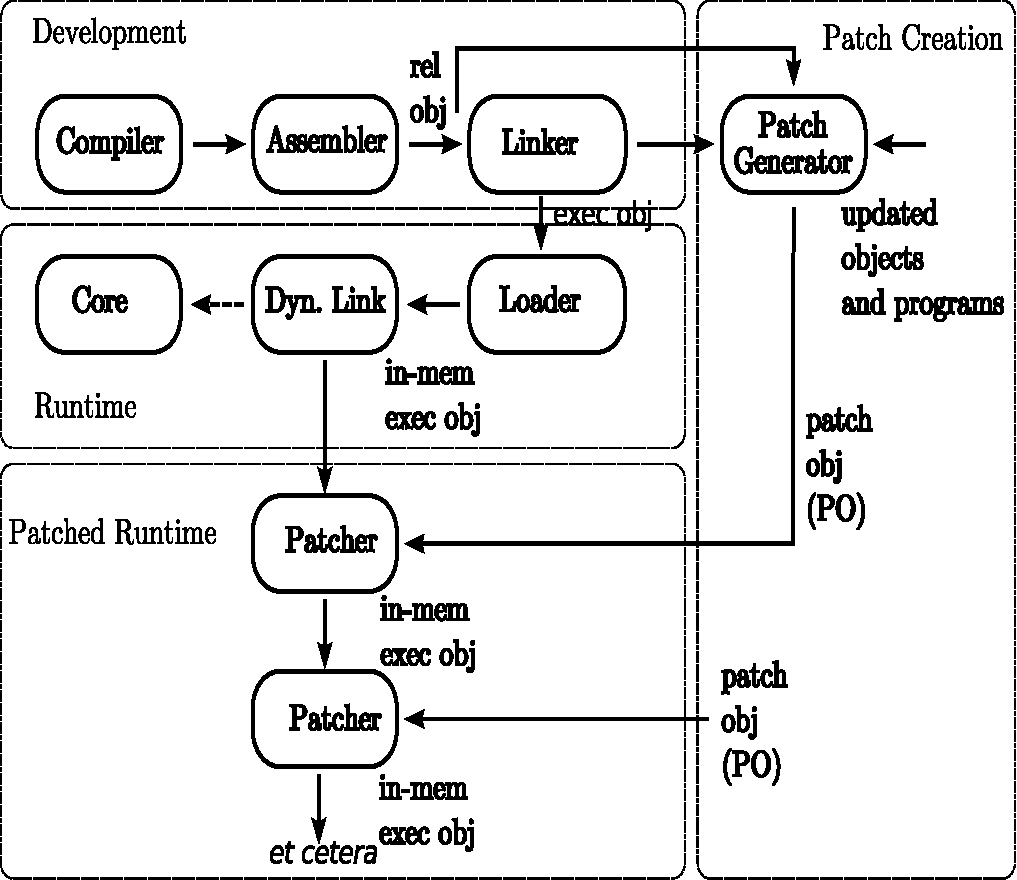
\includegraphics[scale=0.5]{software_lifecycle.pdf}
\end{center}
\caption{{\small Revised software life cycle. Before hot patching, only
    the Development and Runtime portions existed}}
\label{fig:lifecycle}
\end{figure}

% LocalWords:  toolchain


%\subsection{Why Not Just Employ Redundancy?}
{\bf Why Not Just Employ Redundancy?}
\label{ssec:redundancy}

Redundant infrastructure, containing replicas of nodes and service
paths, often helps an organization bridge the service disruption
stemming from patches.  We believe, however, that redundancy isn't
always the best approach for ensuring availability during an upgrade
or security-critical patching process.  Rather than an established
best practice, we invite the reader to see redundancy as
an extreme measure that needlessly duplicates hardware, networking, and
software of the original system. We suggest that redundancy is: 

%Such a mirrored system ensures that service remains
%uninterrupted whenever a {\it failover} is initiated. A {\it failback}
%scenario occurs when the redundant machine hands over control back to
%the original. 

\renewcommand{\labelenumi}{\alph{enumi}.}

\begin{enumerate}
\item {\bf expensive -} especially in medium-sized enterprises where
  the cost of a single server, gateway, or switch is high enough to
  outweigh the benefits of redundancy.

\item {\bf wasteful -} Redundant systems are typically passive
  bystanders, lying in wait for an active machine to
  initiate a failover.

\item {{\bf requires complicated logic -}} Transferring application
  state (even across multiple homogenous systems) is non-trivial,
  especially when the state transfer occurs within hardware (such as
  for call trunks).

\item {{\bf specialized -}} The process of building system redundancy
  is not easily generalizable across heterogenous systems and requires
  full knowledge of the underlying protocol and application state in
  order to provide faithful failover and failback.
\end{enumerate}

It should be noted that the last two items apply even for virtualized
redundant systems, which often do not have the traditional overhead of
redundant hardware.  We do not claim that redundancy does not have its
place, but redundancy does not provide the easy, ubiquitous solution to
high-availability stateful applications which we hope to provide
through patching

% LocalWords:  stateful virtualized


\section{Katana Design}
\label{sec:design}

In our prototype, a patch is may be generated as follows. The source
directory corresponding to the target to be patched is replicated, and
the source code is patched to the version desired. The modified source
tree is then built and compared with the original source tree at the
object (.o) level. Those object files that have changed between the
modified and original source trees are added to the list of objects
that must be examined for type and code transformations. Future work
will include use of the {\it inotify} mechanism to avoid potentially
expensive recursive directory comparison and provide more precise
notification of changed files.

% Katana leverages the typical Unix {\tt Makefile} build mechanism to track
% file-level dependencies.  Normally, after applying a source patch file
% and performing a top-level {\tt make}, only those object files whose
% underlying sources have changed are rebuilt.  Katana thus tracks
% object-level (.o) dependencies as follows.  We first replicate all
% object files and the ELF executable from the existing source tree.  We
% then apply the patch to the {\it original} source tree.  At this
% point, only source files have been modified. Next, using the Linux
% kernel's {\it inotify} mechanism\footnote{{\it inotify} allows the
%   registration of filesystem triggers. We use inotify to avoid potentially
%   expensive recursive directory comparisons.}, Katana sets up a notification
% on the original source tree, so that it knows when an object file is
% created or modified under the original tree.  Finally, we perform the
% top-level {\tt make} under this source and record all created/modified
% object files, along with the newly created executable. The use of
% inotify is not inherent to our general patching mechanism, and indeed
% our present prototype only compares two directory trees and examines
% all object files.

\begin{figure}[ht]
\begin{center}
\includegraphics[scale=0.25]{making.pdf}
\end{center}
\caption{{\small {\it An Example Code Base.} From the top: each source
    file creates a corresponding object file; multiple object files
    are combined into intermediate compilation units (CU); and
    multiple CUs are merged to form the executable. All shaded blocks
    indicate modified files.}}
\label{fig:making}
\end{figure}

%reworded to how we're actually doing it now
% Figure~\ref{fig:making} illustrates how object files are modified by
% {\tt make} as a result of source-level changes.  Katana only considers
% objects that are closest to the source files and ignores all other
% intermediate object files and compilation units (CU).  Hence, in
% Figure~\ref{fig:making}, Katana only records the shaded circle-objects
% along with the final executable.

To dynamically update the running application, Katana needs to patch
both the {\bf code} and the {\bf data} within the process.  It first
creates a {\it patch object} (PO): an ELF file with sections that
indicate the type of patch (code or data), the patch offsets and
lengths within the process address space, patch data, function and
data names, {\it etc}. The patch object may then be applied to the
target at any time.
%The following sections explain how Katana
%handles both code and data patching.


\section{Automated Patching}

In this section, we describe our data and code patching methods.  We
note that, compared to previous work, our PO data structures
allow reasoning about the scope, extent, and impact of the patch ({\it
 e.g.,} whether it affects particular subsystems within the process).

%\subsection{Code Patching}
{\bf Code Patching.} %\hskip 0.1in
This process involves several stages.
%\newline
\newline
(i) {\it Code Identification:} Katana first needs to identify the
section(s) of text that need to be modified within the running
process. To do this, we consider the list of all modified object files
from our tracking step, and identify all functions (both static and
global) within these files 
%SB:
from their symbol table. 
%JMHO: removed talk of copying all functions
Functions that differ between the original
and modified versions of an object file are copied into the PO and
marked as code.
%\newline
\newline
(ii) {\it Symbol Resolution:} After identifying all functions that
require a patch, we need to resolve outstanding symbol references
within each function. Typically, symbol resolution for an application
happens at both the linking stage (called {\it static linking}, when
the symbol is present within another object file or archive), and the
execution stage (or {\it dynamic linking}, when the symbol is present
within a shared library).  All code relocations are identified in the
ELF sections {\tt .rel.text} and {\tt .rela.text}, within the object
files and the final executable.  Each relocation entry contains, among
other information, the code offset that requires relocation, and the
outstanding symbol that provides this fix-up.

For each relocation entry, Katana copies the corresponding symbol into
the PO. The actual value of the symbol is not necessary in the PO
unless the target to be patched will be stripped, as the value of the
symbol can be retrieved from the running target while performing the
patching. This is key in allowing executables which have already been
patched to be patched again.
%Katana uses the replicated executable (from
%{\it before} the patch) to figure out the address of the symbol.  If
%the symbol was provided by another object file, then the symbol table
%of the old executable contains this final address, and we update the
%PO accordingly,
%SB:
%with this address as the patch target. 
If the symbol was
dynamic ({\it i.e.,} present in a shared library such as {\tt libc}),
then the fixup value is the address of a corresponding entry in the
procedure linkage table ({\it PLT}) of the executable.  The PLT is
essentially a jump table with entries for each symbol that needs to be
resolved at runtime by the dynamic linker.  When the process begins
execution, the dynamic linker maps the required shared libraries into
the address space of the process, and updates each PLT entry.

For dynamic symbols, Katana traverses the PLT entries of the
executable and compares the symbol name of each entry with
the symbol name that requires relocation. Once a match is found, the
symbol value can be determined. In our prototype,
Katana is unable to handle calls to previously
%SB:
unused functions present in any shared libraries\footnote{This would
  require creation of new PLT and GOT entries and either subsequent
  re-basing of the following segments of the executable, or creation
  of a new segment to allocate the extra entries. Although ELF
  rewriting systems like ERESI or Diablo show that such manipulations
  can be made practical, we chose not to complicate Katana with
  them yet.}
, although support for this is planned.

Finally, if the outstanding symbol's definition was not found within
the replicated executable (either within the symbol table or the PLT),
then it was newly added by the patch; it is marked as such and added
to the PO.
%\newline
\newline
(iii) {\it Patch Application:} Applying a code patch is simple enough,
and has been researched in other
systems~\cite{pannus,livepatch,ksplice,kaho}.  We map the new function
in memory, and insert a trampoline {\tt jmp} instruction at the
beginning of the old function within the process memory image. This
interposition allows the caller to execute our new function instead of
the previous one at the cost of an extra jump.  It is possible to
avoid the overhead (from branch mis-prediction) of the {\tt jmp}
instruction by adding code in the old function which traces up the
stack and modifies the caller's {\tt call} instruction operand to
point to the new address instead of the old one. Although this
optimization would ensure that all subsequent calls from the same
caller would execute the new patched function without stepping into
the old one, it does makes the process of rolling back a patch
non-trivial. A simpler method to avoid the overhead would be to
relocate all calls to the function to point to its new definition
(although the trampoline would still be desirable, to catch calls from
function pointers or anything of similar nature). The current
prototype uses only the trampoline method.

%\subsection{Data Patching}
{\bf Data Patching.} %\hskip 0.1in
Patching data within a running process is significantly harder than
patching application code.  The primary challenge here is to
synchronize the code and the data structures it acts on.\footnote{For
  example, consider adding a new member to a C struct definition and
  an additional clause to the logic that processes it.}

Tracking down previously allocated data is nontrivial (one of the
reasons why garbage collectors are interwoven with the language
implementation).  Even after identifying the allocated chunks of
memory, in the absence of some kind of a type specification, the {\it
  internal structure} of memory remains opaque.  We also need a method
for extracting only the modified data variables from the patch and a
means to discover the actual modifications that were performed. 
%JMHO: added the below because otherwise I don't think it's clear we
%solved them
Our system solves both of these problems.

We first note that any code that acts on patch-modified data is
already taken care of by Katana's code patching process. This is
because we rely on {\tt make} to build the object files that
correspond to all modified sources. We resolve the previously
identified problems towards patching data by leveraging
DWARF\footnote{\url{http://dwarfstd.org}} debugging information within the
application executable. This requires the object files to be compiled
with debugging support, but we do not see this as a limitation. Since
we only need DWARF information while building the PO, all debugging
symbols could be stripped from the executable during application
deployment, if so desired 
%JMHO:
(this would require storing symbol values in the PO, however).
%JMHO end
We recall the representation of types in
the DWARF format and then detail the various steps in Katana's data
patching process.

{\bf DWARF type information.} %\hskip 0.1in 
The DWARF structure is laid
out as a tree of DIEs ({\it Debugging Information Entries}) within the
executable file. Each DIE has an associated tag and a set of
attributes. The DIE that defines type information has the tag as one
of {\tt DW\_TAG\_base\_type}, {\tt DW\_TAG\_structure\_type} or {\tt
  DW\_TAG\_union\_type}. Typedefs and other type modifiers (such as
{\tt const}, {\tt volatile}, {\tt pointer} {\it etc.}) are referenced
by the DIE that defines the type. In case of structures or unions,
each member is contained as a separate DIE within the parent DIE that
identifies the struct/union. It is important to note that DWARF
annotates types of {\it all} visibilities from the program sources -
local, global and static.

Katana's data patching process contains a number of steps:

(i) {\it Type Discovery:} We set out to discover all newly created or
modified data types -- those that are primarily user-defined (such as
structures and unions in {\bf C}). Katana traverses the type information
(as identified by the above DWARF tags) from the newly created executable,
 and for each encountered type, it searches for
the corresponding type-name within the {\it replicated} executable
(from before the patch). If so found, the full types (i.e. the number,
type and position of all member variables contained within) are
compared to determine if they are identical. If not identical,
a transformation between the old and new versions is generated, along
with DWARF information identifying the type to insert into the PO as
soon as a variable is found making use of the altered type.
%the parent type identifying the struct/union is inserted into the PO.
 Else, if
the type name itself was not found within the replicated executable, then the
current type was created by the patch, and is added as such to the PO.
%\newline
\newline
(ii) {\it Data Traversal:} The next step is to traverse all variables
defined within the new application, and for each one encountered,
we first determine its 
%SB:
lexical scope.
If the scope is
local, then we ensure that the corresponding function (the one that
defines this variable) does not have an activation frame on  
the program stack while
applying the patch. Else, the variable has been defined as either
global or static. We first check if the replicated executable defines
the same variable. If not, then this variable has been created by the
patch and we need not worry about it and leave the symbol resolution upto
the compiler (as only {\it new} code can use this variable). Otherwise,
we verify whether the variable's type is one of the
modified types identified during {\it type discovery}. If it is, then
we add the variable along with its {\it original} address from the replicated
executable, its {\it new} address from the patch, and type information to the
PO. At the end of this stage, Katana would have identified all newly
created or modified variables from the patch. Dealing with variable
scope and safety is still a work in progress in the current prototype.
%\newline
\newline
(iii) {\it Patch Application: } Applying a data patch consists of
first tracking down the relevant symbols in program memory. Katana
reads in the PO, and for each data variable encountered, it checks if
the variable is a pointer or not. If it is, then the current validity of the
pointer is verified (by bounds-checking the pointer value to within
heap boundaries).  If the pointer is found to be invalid, no further
action is taken.  If the pointer is valid, then memory for the new
type(s) is allocated, the older structure is copied into the new one
taking into account the difference in structure definition, the old
memory is then freed, and the pointer is modified to point to the new
segment (in case of structures such as lists, trees, since we have the
type specification, we can repeat this process recursively for each
node on the list or tree). Else if the variable is not a pointer, then
Katana modifies all its references in the program text to the updated
memory location from the patch. In the current prototype, Katana
automatically zeros all {\it new} member variables within structures.
Eventually it will support default values and programmer-written
custom initializers.

{\bf Challenges.} %\hskip 0.1in 
Hot patching still faces a number of
challenges, including dealing with multithreaded programs and address
space randomization (which slight changes to the OS loader can help us
overcome).  
There is nothing inherent in our design which will not work with
multithreading, but dealing with it through ptrace takes considerable
work which we have not yet done.
Furthermore, dynamic updates require some knowledge of the
program's execution state so that the application is quiescent with
respect to the code and data being altered by Katana as it applies the
Patch Object. 
% We consider the program to be in a safe state if all
% activation records are free of functions contained in the PO and all
% activition records are free of functions that $(1)$ access any global
% or static symbols we identify during Katana's {\it Data Traversal} stage and
% $(2)$ do not define any local variables of modified types identified
% during our Type Discovery phase.  Katana uses the {\tt ptrace}
% interface to pause execution and query this state.
%
%JMHO: We repeat this again in the discussion section, so I commented
%it out here and added a brief note saying we discuss it more below
We have not
yet implemented a safety determination mechanism, but we discuss our
approach to it in the next section.

% LocalWords:  ptrace multithreading JMHO


\section{Discussion}

{\bf When to apply the patch.}
%
Dynamically updating a running application requires diligence and
patience. One cannot update the target application without any
knowledge of the program's execution state, by which we mean the
program stack, processor registers {\it etc}.  Even after possessing
this information, the application has to be in what we call a ``safe
state'' for Katana to apply the patch. We characterize a program state
as a {\it safe state} if the following two conditions hold:
\begin{itemize}
\item All activation frames in the program stack belong to functions
  that {\it do not} get updated during code patching. It is easy to
  verify this by comparing each function on the stack to the list of
  upgradeable functions contained within the PO.

\item All activation frames in the program stack belong to functions
  that do not access any global/static symbols identified during {\it
    Data Traversal}, and do not define any local variables of the
  modified types identified during {\it Type Discovery}. Again, since
  we maintain type and variable definitions within the PO, verifying
  this condition is easy.
\end{itemize}

Given the patch object, Katana uses Linux's {\tt ptrace} interface to
temporarily halt the execution of the target process, query the
current execution stack and determine if the application is currently
in a safe state. If so, then Katana applies the code patch followed by
the data patch. We note that it is not possible to apply the code and
data patches at different times since new code likely uses the new
data, and hence postponing data patching to when only the second
condition is satisfied is impractical and unsafe.

Let $A$ denote be the current activation frame on the program stack,
and the notation $(X:Y)$ define all frames from $X$ to $Y$ (on a time
scale, $X$ precedes $Y$) on the stack; so $(1:A)$ defines the current
stack. Now, in case we determine $(1:A)$ to be an unsafe state, we
could repeatedly keep querying the stack until the application reaches
some safe state. However, this is highly inefficient and cumbersome.


Instead, when we determine the program to be in an unsafe state, we
traverse up the stack from $A$, and for each preceding frame (say
$A'$), we determine if $(1:A')$ is a safe state. This takes into
consideration only $A'$ and all other frames preceding it. If $(1:A')$
is a safe state, then we insert a breakpoint on the return instruction
pointer ({\tt EIP}) pointed to by the successive frame: $(A' +
1)$. What this guarantees us is that when this breakpoint is hit, the
state of the program stack will be $(1:A')$. Since we just determined
this to be a safe state, we can reliably conduct the patching
procedure. If however, no such frames preceding $A$ satisfy a safe
state, then it means that the application cannot be patched
successfully in its current execution since there will always be a
function that violates our safety condition.

Finally we note that even after inserting a breakpoint, the problem of
determining {\it when} the breakpoint will be hit is essentially a
hard one, and so in such cases, Katana can provide no time-bounding
guarantees. Still, this is a cleaner and more efficient approach than
just na\"{i}vely retrying the full update procedure, which is both an
expensive and incomplete solution.
%JMHO:
In cases where the timely (or even eventual) application of a patch
seems unlikely, it would be possible to add support for programmers to
manually specify safe places for patching to occur. For programs built
around a central loop (the vast majority of long-running programs),
the likelihood of safe patching can be expedited by isolating the main
loop into a simple routine unlikely to ever need patching. While
safety determination is implemented in our prototype, we do not yet
have enough real data about the likelihood of applications failing to
reach a safe state.
%JHMO end

%\subsection{Multithreading}

{\bf Address Space Randomization.}
%
{\em Load-time address randomization} has become a stable and popular
way of raising the bar for attackers, and so we must discuss how it 
interacts with our patching scheme. 
%
The gist of randomization schemes is invalidating various default
assumptions regarding the locations of code and data elements that
might facilitate exploitation.
%
%
%SB: condense
% ``Randomization''\footnote{We note that gist of this defense is not
%   randomness as such, but rather increasing the targets' diversity,
%   and denying the convenience of ``code once, run everywhere'' to the
%   attackers.}  is usually the task of the loader and the dynamic
% linker, which, at the time when a process' virtual address space is
% created or new code is loaded into it, modify its layout from the one
% prescribed by the linker that created the original executable's ELF
% structures. In particular, the virtual addresses of loadable segments
% in the file are shifted by a random\footnote{In reality, the choice of
%   offset is still limited by the platform's alignment requirements}
% offset.  This implies that the loader must perform {\em relocation},
% and indeed the code that can be so treated must be accompanied by
% relocation sections.
%
In particular, the virtual addresses of loadable segments
 are displaced by random\footnote{In reality, the choice of
   offset is still limited by the platform's alignment requirements.}
offsets by the loader, which {\em relocates} them (using their
accompanying relocation sections).
% The sections that can be so treated must be accompanied by
% relocation sections.

Patching %``randomly'' 
relocated code with our PO files requires
knowledge of the displacements introduced at loading-and-relocation
time. While there is no common ABI standard for saving this
information, conceptually it is no different from saving virtual
addresses of other files' loaded symbols in the {\it Global Offset Table}
(GOT). We note that the names of the constituent object files themselves 
are customarily included in the symbol tables, and that the symbol
table entry format can be easily adopted for storing virtual addresses
of the %``randomly'' 
relocated objects.

Thus, at the cost of small modifications to the OS loader and the 
dynamic linker, we can make the information on the layout of the
``randomly'' relocated executable and libraries available to
our patching process driven by our POs.\footnote{We note that saving 
this information 
%
about the post-relocation layout of the process 
does not weaken ``randomization'', because 
the latter does not assume the attacker's ability to arbitrarily read 
process memory (in which case the addresses of required symbols are
easily found by scanning it %). %
for their code or data patterns), 
but rather breaks hard-coding of these symbols' expected addresses.
} 

{\bf Future work.} Katana is a work in progress.
%JMHO:
We have demonstrated code patching (including dynamically linked
functions), the use of our patch object format (discussed in detail in
Section \ref{sec:poformat}), and data patching including complex
structures and variable addition. The remainder of the system is still
under development. In the future we
%JMHO end
must address several 
important engineering issues, such as interaction of patched code with
dynamically loaded libraries (including the {\em dlopen} mechanism),
and assuring that accumulation of administered patches does not lead to
unacceptable performance degradation. It also poses a broader question
of describing and detecting software designs not amenable to its runtime
patching and steering programmers to avoid them if possible. 


\section{Patch Object Format}
\label{sec:poformat}
%\subsection{Reasons and Needs}
{\bf Reasons and Needs.}
We have developed a Patch Object format for which the following holds:
\begin{itemize}
 \item A PO is a valid ELF file.
 \item A PO utilizes DWARF information to describe types, variables, and functions requiring patching.
 \item A PO allows type transformations to be specified using a language defined by the DWARF standard.
\end{itemize}
Through the use of existing standards and well-structured ELF files
utilizing a simple expression language for data patching, we aim to
create patches that are easily examined (or modified) with existing
tools. This easy compatibility with the existing binary tools and
standards brings us to a very good point: why should patching not be a
part of the ABI and of the standard toolchain? This does not
necessarily have to be the precise format we use for Katana. Any such
format that would become a standard, whether an actual standard or a
de-facto standard, should be well vetted by the community, but we argue
that something like this should be included in the standard object
types, along with relocatable objects, executable objects, shared
libraries, and core dumps. Consider the situation. Relocatable objects
containing new code and data which may be inserted at runtime are
nothing new. This is the entire premise of the dynamic
library. User-written functions which may have to run upon this code
injection (in the case of patching data where the desired actions
cannot be determined automatically) already exist as the
\texttt{.init} and \texttt{.fini} sections. Because of this similarity
between some of the functionality needed by patching and the
functionality offered by dynamic
libraries, some previous systems have performed patching by creating
patches as dynamic libraries that contain not only the code and data
to be patched but also the mechanism to perform the patching \cite{ginseng}
\cite{polus}. We argue that
this is an unnecessary mixing of data and logic and, further, that a patch
that contains merely the information necessary to fix a running
process and not the code to do so is more desirable. The code to apply
the patch should live in one place on any given system, as most other
executable content does. We do not embed Emacs within our text files,
after all. Dynamic libraries and other relocatable, linkable objects
do not contain code and data intended to overwrite data in an existing
executable or process. Consider, however, that redefining certain
symbols is only a slight twist on ordinary linker behaviour. Ordinary
linker behaviour for global symbols is to fail if a symbol is defined
more than once. Ordinary behaviour for weak symbols is to use a global
definition if available or the weak symbol otherwise. When performing
dynamic linking, generally the first appropriate symbol encountered in
the chain of symbol tables is used. It is not a far difference to
define the linkage rule that the symbol definition from the most
recent patch takes precedence. Therefore, applying a patch consists of
the following steps
\begin{enumerate}
\item Injecting appropriate sections of the patch into memory. This
includes putting their contents into memory and performing relocations
on these sections (but not on the rest of the in-memory process) so
that they fit into their environment
\item Copying existing data to the appropriate regions of the newly
mapped-in patch
\item Performing relocation on the entire in-memory process such that the
symbols defined by the patch take precedence.
\end{enumerate}
These steps are all such fundamental operations that they should
become universally supported by the ABI and the toolchain. 

On the other hand, note that the specification of a general patch
format does not completely prescribe the patch application. From a
standard patch format, a patcher is still free to make decisions such
as when to patch safely and whether to patch functions by inserting
trampolines in the old versions of the functions or by relocating all
references to the function (we currently do the former in Katana, but
may later transition to doing the latter).

%\subsection{Our Patch Object Format}
{\bf Our Patch Object Format.}
Our Patch Object (PO) format is an ELF-based format. Figure
\ref{fig:elfheaders} shows the sections contained in a simple
patch. \texttt{.text.new} and \texttt{.rodata.new} are of course the
new code and supporting

%\begin{wrapfigure}{l}{0.4\textwidth}
%{\footnotesize
\begin{figure}[ht]
\begin{center}
\begin{verbatim}
  Section Headers:
    [Nr] Name              Type          
    [ 0]                   NULL          
    [ 1] .strtab           STRTAB        
    [ 2] .symtab           SYMTAB        
    [ 3] .text.new         PROGBITS      
    [ 4] .unsafe_functions LOUSER+1
    [ 5] .rodata.new       PROGBITS      
    [ 6] .rela.text.new    RELA          
    [ 7] .debug_info       PROGBITS      
    [ 8] .debug_abbrev     PROGBITS      
    [ 9] .debug_frame      PROGBITS      
    [10] .rel.debug_info   REL           
    [11] .rel.debug_frame  REL           
\end{verbatim}
\end{center}
%}
\caption{Headers for the PO}
\label{fig:elfheaders}
%\vspace{-10pt}
%\end{wrapfigure}
\end{figure}
constants to inject. \texttt{.rela.text.new} allows \texttt{.text.new}
to be properly relocated after it is adjusted. While System V based
systems use only relocation sections of type \texttt{SHT\_REL}, we
chose to use \texttt{SHT\_RELA} in our patch objects because they make
addends much easier to keep track of as we relocate from patched
binary to patch object to patched process in memory. This is all
really nothing new; storing ELF sections to be injected in-memory has
been done before in other systems \cite{eresi}. What is new in our patch object is
the inclusion of DWARF sections. The \texttt{.debug\_info} section in
an ordinary executable program contains a tree of DIEs (Debugging
Information Entities) with information about every type, variable, and
procedure in each compilation unit in the program. In a patch object,
we store information only about the procedures and variables which
have changed. This of course includes storing the type information for
changed variables. An example of the DWARF DIE information contained
in a patch can be seen in Figure \ref{fig:dies}.

Note that we store considerably less information about each entity
than is typically contained. This is so because we read most of the
information from the DWARF and symbol table information of the
executing process (unless it will have been stripped; then more
information must be stored in the patch). This allows the patch to be
more flexible as it does not require that all variables and procedures
be located at exactly the addresses they were expected to be at when
the patch was generated. This flexibility allows a single patch
between versions \emph{va} and \emph{vb} to patch both an executable
that was originally compiled to \emph{va} and an executable that was
patched from earlier versions to be equivalent to \emph{va}. Ksplice,
one of the few other patchers that operate solely at the binary
level, does not have this capability \cite{ksplice}. We will provide a
mechanism for composing patches such that a patch from version
\emph{va} to \emph{vb} may be composed with a patch from \emph{vb} to
\emph{vc} to produce a patch from \emph{va} to \emph{vb}. Note that
patch versioning is currently a work in progress and not fully
implemented.
%\begin{wrapfigure}{r}{0.5\linewidth}
\begin{figure}[ht]
{\small
\begin{center}
\begin{verbatim}
  .debug_info

  COMPILE_UNIT<header overall offset = 0>:
  <0><   11>	DW_TAG_compile_unit
      DW_AT_name                  main.c

  LOCAL_SYMBOLS:
  <1><   19>	DW_TAG_subprogram
      DW_AT_name                  printThings
      DW_AT_low_pc                0x0
      DW_AT_high_pc               0x70
  <1><   40>	DW_TAG_structure_type
      DW_AT_name                  _Foo
      DW_AT_byte_size             16
      DW_AT_MIPS_fde              16
      DW_AT_sibling               <93>
  <2><   55>	DW_TAG_member
      DW_AT_name                  field1
  <2><   63>	DW_TAG_member
      DW_AT_name                  field_extra
  <2><   76>	DW_TAG_member
      DW_AT_name                  field2
  <2><   84>	DW_TAG_member
      DW_AT_name                  field3
  <1><   93>	DW_TAG_base_type
      DW_AT_name                  int
      DW_AT_byte_size             4
  <1><   99>	DW_TAG_variable
      DW_AT_name                  bar
      DW_AT_type                  <40>
\end{verbatim}
\end{center}
}
\caption{DWARF DIEs in the PO}
\label{fig:dies}
\vspace{-10pt}
\end{figure}
%\end{wrapfigure}

Most of the information in the DIE tree is concerned only with names
or how to locate code within the patch object (high and low pc). Of
special interest, however, is the \texttt{fde} attribute of the
\texttt{DW\_TAG\_structure\_type}. This attribute specifies an offset
in the \texttt{.debug\_frame} section of an FDE (Frame Description
Entity). DWARF FDEs are designed for use in transforming one call
frame into the previous call frame, and thereby walking up a call
stack for either debugging purposes or exception-handling purposes
(using the \texttt{.eh\_frame} section). Transforming one call frame
to another, however, is not such a different operation from
transforming one structure to another version of the same
structure. We have aided this use with an implementation of the DWARF
virtual machine that defines several special register types
(exploiting the fact that for the purposes of generality, DWARF
registers are specified as LEB128 numbers, giving an unlimited number
of registers). The DWARF register instructions contained in the FDE
referenced in Figure \ref{fig:dies} for copying \texttt{field1}, \texttt{field2}, and
\texttt{field3} from the original version of a structure \texttt{\_Foo}
to a new version of \texttt{\_Foo} that has gained the extra member
\texttt{field\_extra} in the middle of the existing fields would be
represented as in Figure \ref{fig:fdeinstrs}.
\begin{figure*}[ht]
{\small
\begin{center}
\begin{verbatim}
DW_CFA_register {CURR_TARG_NEW,0x4 bytes,0x0 off} {CURR_TARG_OLD,0x4 bytes,0x0 off} 
DW_CFA_register {CURR_TARG_NEW,0x4 bytes,0x8 off} {CURR_TARG_OLD,0x4 bytes,0x4 off} 
DW_CFA_register {CURR_TARG_NEW,0x4 bytes,0xc off} {CURR_TARG_OLD,0x4 bytes,0x8 off} 
\end{verbatim}
\end{center}
}
\caption{FDE instructions for data patching}
\label{fig:fdeinstrs}
\end{figure*}

\texttt{CURR\_TARG\_NEW} and \texttt{CURR\_TARG\_OLD} are special
symbolic values defined by the virtual machine. If we are patching the
variable \texttt{bar}, then the \texttt{CURR\_TARG\_OLD} will be the old address of \texttt{bar}
(its value in the symbol table), and \texttt{CURR\_TARG\_NEW} will be the new
address bar is being relocated to. Our registers take advantage of the
LEB128 encoding to hold a considerable amount of information in the
register identifier. In the case seen above, the first byte identifies
the class of the register (\texttt{CURR\_TARG\_NEW} or \texttt{CURR\_TARG\_OLD} in this
example), the following word specifies the size of the storage
addressed (this is included so that register assignments may copy an
arbitrary number of bytes), and the final word specifies an offset
from the address referred to by \texttt{CURR\_TARG\_}(\texttt{NEW}|\texttt{OLD}).

% LocalWords:  toolchain linkable init fini FDE FDEs DIEs Polus CURR TARG LEB
% LocalWords:  CFA DW Foo


\section{Related Work}
\label{sec:related}

There are several hot-patching systems preceding Katana. One of the
most well known is probably Ginseng \cite{ginseng}. Ginseng (and
systems drawing inspiration from it such as Polus \cite{polus}) have
successfully demonstrated patching of such important software as
apache and sshd. These systems perform analysis of the differences
between the original and patched versions at the source code
level. This introduces considerable (and we argue unnecessary)
complexity and inability to deal well with some optimizations such as
inlining and hand-written assembly. The complexity of analyzing the
source code ties these systems to generally a single language (C in
the case of both Ginseng and Polus). By contrast, Katana is language
agnostic as it works at the level of the binary ABI, and although we
have not yet demonstrated it doing so, it should eventually be able to
patch binaries compiled from any language, providing the necessary
symbol and relocation information is supplied. Ginseng also requires
significant programmer interaction in annotating the code
\cite{ginseng-manual} and requires compiling the code to use
type-wrappers, allowing the patching of data types but at the cost of
indirect access to them. The more programmer effort involved in
generating a patch, the more likely the patch is to be incomplete or
incorrect.

Motivated by many of the points in the above paragraph, the
successful Ksplice system \cite{ksplice} patches at the binary level, as we do. We
claim the following differences from and improvements over Ksplice.
\begin{itemize}
\item Ksplice operates on the kernel. As their paper states, most of their
  technique is not specific to the kernel, but there is no evidence
  that it has been implemented to function on userland programs.
  Katana operates on userland.
\item Ksplice makes no attempt to patch data, relying entirely on
  programmer-written transformation functions when data types do
  change
\item Ksplice patches are created as kernel modules. Ksplice does not
  provide a mechanism to perform operations, such as composition,
  on these patches.
\end{itemize}

To the best of our knowledge, Katana is the first system to utilize
DWARF type information in patching.

Maintaining continuous availability, even in the absence of disruptive
events like patches, is both a challenging technical exercise and the
driving need for research on dependability, reliability, and fault
tolereance~\cite{deltaexec}. 
%The work most closely related to Katana focuses
%JMHO: reworded above because I don't think this is what's most
%closely related
Our work follows work focusing
%JMHO end
 on enabling a software
application to continue providing service or survive significant
events like errors, exploits, and patches.  This body of work includes
research on dynamic kernel updates, software survivability, and
software self-healing. However, other research areas also addressed the
challenge of enabling software to adapt at runtime, e.g., the area
of software evolution (e.g.,~\cite{software-evolution}).

The concept of crash-only software~\cite{crashonly} advocates
microrebooting: the procedure of retrofitting each component of a
system with the ability to crash and reboot safely as the default mode
of operation.  Despite its appeal as a design principle, such an
approach would be difficult to retrofit to legacy software.
Although restarting a particular service or application is disruptive
enough, rebooting the operating system itself multiplies this
disruption.  
The need to avoid that kind of downtime helped drive the
creation of frameworks like Loadable Kernel Modules for Linux, which
allow for extending the kernel during runtime without a reboot.
The ability to update the running kernel (as opposed to adding
or removing modules) without rebooting was achieved at least ten years
ago~\cite{cesare1998} and recently rediscovered, albiet mostly for
research, rather than commodity,
kernels~\cite{nonLKMkernpatch,baumann2007osupdate,soules2003k42}).
Even so,
dynamic updates of the kernel during runtime that don't require a
reboot are difficult to apply to a commodity OS, although several
efforts have been successful for the K42 experimental
system~\cite{soules2003k42,baumann2005k42}.

Software self-healing aims at ensuring continuous or increased
availability for systems subjected to exploited vulnerabilities,
either by automatically generating
patches~\cite{weimer2009genetic,stelios2005usenix} to gradually harden
the application or seeking to avoid a restart altogether by modifying
certain runtime aspects ({\it e.g.,} the memory
subsystem~\cite{rinard2004osdi}, properties of the execution
environment~\cite{rx2005sosp}), 
%
or selected control
paths~\cite{dira2005,locasto2007usenix}) of the system in response to
attacks.
One major risk of employing self-healing in production environments is
that the semantics of follow-on execution remain largely uncontrolled,
although recent work in automatically correcting memory
errors~\cite{exterminator2008cacm} seems to achieve fairly reliable
results.  Both automated responses and traditional patches can make it
difficult for an administrator to understand the implications of a
particular fix~\cite{rinard.ppp}.

\section{Conclusion}
\label{sec:conclusion}

We introduce a method for hot patching: a technique we believe to be a
promising alternative to redundancy, ad hoc self--healing techniques,
``patch and pray,'' or other approaches to dynamic software updates.
Hot patching has the potential for aligning actual practices with
acknowledged ``best practices'' relating to critical security or 
functionality updates.  We hold that one major impediment to hot
patching is the opaque nature of most patches (be it
proprietary or open software), and our method of patching along with the
PO file format are first attempts at providing a basis for informed reasoning
about the structure and implications of a patch. 

We present a reasoned approach to making patching a part of the
standard tool chain. We demonstrate a working binary userland patcher
operating completely at the object level. Our system is, to our
knowledge, the first to utilize DWARF type information to automate the
transformation between old and new versions of a type. There yet
remains much work to be done, and our future work involves support for
patching multithreaded targets, better support for handling opaque
types such as \texttt{void}*, and further development of patch
versioning and the ability to perform operations on patch objects.


% Now in \thanks in author list.
%% superceded by \thanks in header
\section*{Acknowledgements}

{\small 
The first three authors' work was supported in part by the National
Science Foundation, under grant CNS-0524695.  The views and
conclusions do not necessarily represent those of the sponsors.
%
Locasto is supported in part by grant
2006-CS-001-000001 from the U.S. Department of Homeland Security under
the auspices of the I3P research program. The I3P is managed by
Dartmouth College. The opinions expressed in this paper should not be
taken as the view of the authors' institutions, the DHS, or the I3P.
}


{\small
%\bibliographystyle{apa-good}
\bibliographystyle{abbrv}
\bibliography{locasto,extras,oakley}
}



\end{document}
